%%%%%%%%%%%%%%%%%%%%%%% file template.tex %%%%%%%%%%%%%%%%%%%%%%%%%
%
% This is a general template file for the LaTeX package SVJour3
% for Springer journals.          Springer Heidelberg 2010/09/16
%
% Copy it to a new file with a new name and use it as the basis
% for your article. Delete % signs as needed.
%
% This template includes a few options for different layouts and
% content for various journals. Please consult a previous issue of
% your journal as needed.
%
%%%%%%%%%%%%%%%%%%%%%%%%%%%%%%%%%%%%%%%%%%%%%%%%%%%%%%%%%%%%%%%%%%%
%
% First comes an example EPS file -- just ignore it and
% proceed on the \documentclass line
% your LaTeX will extract the file if required
\begin{filecontents*}{example.eps}

gsave
newpath
  20 20 moveto
  20 220 lineto
  220 220 lineto
  220 20 lineto
closepath
2 setlinewidth
gsave
  .4 setgray fill
grestore
stroke
grestore
\end{filecontents*}
%
\RequirePackage{fix-cm}
%
\documentclass[smallcondensed,natbib,apacite]{svjour3}       % onecolumn (second format)

\smartqed  % flush right qed marks, e.g. at end of proof
\usepackage{graphicx}
\usepackage{makecell}
\usepackage{multirow}
\usepackage[T1]{tipa}
\usepackage{hyperref} % for urls
\usepackage{float} % force tables in appendices in place
\usepackage{indentfirst} % force first paragraphs of each section to ident
\usepackage{setspace} % double space throughout
\doublespacing

% Insert the name of "your journal" with
 \journalname{Attention, Perception, \& Psychophysics}
%
\begin{document}

\title{Units of processing in perceptual normalization for speaking rate \thanks{This work was supported by National Institute on Deafness and Other Communication Disorders grants T32DC000046 and F32DC019539 (M.C.) and 5R01HD081127 (R.S.N.).}}



%\titlerunning{Rate normalization}        % if too long for running head

\author{Margaret Cychosz\textsuperscript{1} \and
        Rochelle S. Newman\textsuperscript{1}
}

\authorrunning{Cychosz \& Newman} % if too long for running head

\institute{\at \textsuperscript{1}Department of Hearing \& Speech Sciences \\
              University of Maryland, College Park \\
              0100 Samuel J. LeFrak Hall \\
              College Park, MD, 20742 \\
              \email{mcychosz@umd.edu}           %  \\
}

\maketitle

\begin{abstract} 
Because speaking rates are highly variable, listeners must use cues like phoneme or sentence duration to scale or normalize speech across different contexts. Scaling speech perception in this way allows listeners to distinguish between temporal contrasts, like voiced and voiceless stops, even at different speech speeds. It has long been assumed that this normalization or adjustment of speaking rate can occur over individual phonemes. However, phonemes are often undefined in running speech, so it is not clear that listeners can rely on them for normalization. To evaluate this, we isolate two potential processing units for speaking rate normalization---the phoneme and the syllable---by manipulating phoneme duration in order to cue speaking rate, while also holding syllable duration constant. In doing so, we show that changing the duration of phonemes both with unique acoustic signatures (/k\textscripta/) and overlapping acoustic signatures (/w\textsci/) results in a speaking rate normalization effect. These results suggest that even absent clear acoustic boundaries within syllables, listeners can normalize for rate differences on the basis of individual phonemes.

\keywords{speaking rate \and speech perception \and normalization \and speech processing \and categorical perception}
\end{abstract}

\section{Introduction}\label{intro}

Speaking rate varies widely between and within speakers. Yet many phonological contrasts of the world's languages rely on temporal cues, such as vowel length or voice onset time. Consequently, listeners must perceptually \textit{normalize} for speaking rate, remapping acoustic cues across different contexts and speakers, in order to comprehend speech and acquire language. 

Listeners employ perceptual normalization (or compensation) for speaking rate over a variety of levels in the speech signal.\footnote{Throughout the paper, we refer to normalization for speaking rate without implying that listeners normalize for all contextual information during perception. We also do not use the term ``normalization'' to imply that listeners eliminate vs. maintain rate-based information.} For example, to categorize a temporally-cued contrast like /k-g/, listeners could use \textit{proximal} information in the speech signal, like the duration of vowels or consonants that are adjacent to the target phoneme 
\citep{diehlAuditoryBasisStimulus1989,millerEffectsLateroccurringInformation1979,newmanPerceptualNormalizationSpeaking1996,summerfieldArticulatoryRatePerceptual1981}. Listeners could also use \textit{distal} information in the speech signal like the rate of the overall sentential context, another talker's habitual or situational speaking rate, or even the duration of non-speech stimuli like tones \citep{maslowskiHowTrackingHabitual2019, newmanPerceptualNormalizationSpeaking2009,reinischSpeakerspecificProcessingLocal2016,wadePerceptualEffectsPreceding2005}. In both cases, for a contrast like /k-g/, shorter-duration cues (e.g., a shorter adjacent consonant or a faster sentence) suggest a faster speaking rate and therefore bias listeners to the positive voice onset time phoneme /k/. In contrast, longer-duration cues bias listeners to the negative or neutral voice onset time phoneme /g/. 

Research on proximal information for speaking rate normalization has focused on cues such as the duration of phones preceding or following the target segment. As a result, we now know that although there are more degrees of freedom in vowel than consonant duration \citep{crystalSegmentalDurationsConnected1988}, both vowels and consonants can provide rate normalization cues (\citealt{diehlAuditoryBasisStimulus1989,summerfieldArticulatoryRatePerceptual1981}; see \citealt{toscanoCueintegrationContextEffects2012} for an alternative interpretation). Additionally, while more distal cues for speaking rate normalization, like preceding word duration, are well-documented (see previous citations), there is some evidence for an adjacency bias in speaking rate normalization: listeners may only scale for speaking rate over a limited temporal window of a single adjacent phoneme or syllable (\citealt{newmanPerceptualNormalizationSpeaking1996,sawuschPerceptualNormalizationSpeaking2000}; cf. \citealt{baese-berkLongTermTemporalTracking2014}). 

While careful experimental manipulations have led us to understand \textit{which} cues listeners use during perceptual normalization for speaking rate, less is known about \textit{how} the cues are incorporated. This gap in our understanding of rate normalization processes is relevant for a number of theoretical and practical reasons. Research into proximal cues for rate normalization has traditionally assumed that phonemes are the basic unit over which speaking rate can be normalized. But this assumption may be premature. For one thing, it is difficult for listeners to isolate phonemes in the comprehension of spontaneous, running speech. Articulatory undershoot and hypoarticulation reduce phonological contrasts \citep{johnsonHyperspaceEffectPhonetic1993,lindblomExplainingPhoneticVariation1990}. Coarticulation blurs acoustic boundaries between adjacent phones as speakers consistently anticipate upcoming speech sounds \citep{whalenCoarticulationLargelyPlanned1990}. Some phoneme pairs, like glides and vowels or laterals and vowels, are especially susceptible to these coarticulatory pressures and less able to resist the influence of adjacent segments \citep{recasensCoarticulatoryPatternsDegrees1985}. In all, phonemes, particularly voiced, non-strident phonemes, are not reliably discriminable. It is therefore plausible that listeners would instead normalize speaking rates over syllables or other other acoustically-based segments which may not straightforwardly correspond to linguistic representations.

Rate normalization has often been considered a low-level, domain-general auditory process \citep{boskerAccountingRatedependentCategory2017}: it is involuntarily activated after milliseconds of exposure to a speech- or non-speech-like stimulus \citep{reinischSpeakerspecificProcessingLocal2016} and has been documented in non-human (avian) species \citep{welchEffectsSyllablefinalSegment2009}. However, it is also increasingly apparent that several higher-level constructs such as language experience \citep{baese-berkNonnativeSpeakersUse2016}, listener familiarity with the speaker \citep{kleinschmidtPerceptionVariableStructured2016,reinischSpeakerspecificProcessingLocal2016}, and some aspects of language structure such as intonation \citep{steffmanIntonationalStructureMediates2019} also mediate rate normalization. It is thus possible that rate normalization interacts with additional higher-level linguistic units, such as the syllable, although this has not been empirically tested. 

From a machine learning perspective, invariance in the speech signal is a central obstacle to achieving higher-performing speech-to-text and automatic speech recognition applications. Understanding appropriate mechanisms for normalization, including rate normalization, in human listeners may facilitate machine performance, as it may be simpler to program normalization on the basis of acoustically-driven signals (such as syllables) than linguistically-driven concepts (phonemes). If human listeners reliably normalize for speaking rate at the phonemic level, even in the absence of explicit acoustic signals, it would suggest that phonemic structure should be incorporated into natural language processing algorithms to benefit machines' learning of spontaneous speech.  

The present experiments were designed to investigate the effects of acoustic separability, or the ability to distinguish between two adjacent phonemes, on speaking rate normalization. The overarching goal is to understand the processing units (syllable or phoneme) involved in the perceptual normalization of speaking rate. In a pair of phoneme category rating experiments, we asked whether two syllables containing phones differing in acoustic separability (acoustically-distinct /k\textscripta/ versus overlapping /w\textsci/) would result in separate rate normalization effects or in a single combined rate normalization effect. We chose to evaluate the effects of speaking rate upon the perception of the /\textesh -t\textesh/ contrast in American English as this contrast has demonstrated a rate normalization effect in prior research \citep{newmanPerceptualNormalizationSpeaking1996}. In that work, the authors were able to trigger a /\textesh-t\textesh/ phonetic boundary shift in a nonce word series ranging from /\textesh k\textscripta s/ - /t\textesh k\textscripta s/ (``shkas'' to ``chkas'') by adjusting the duration of /k/ in the stimuli. Ambiguous stimuli, with a longer /k/ duration, suggested a slower speaking rate and biased listeners to perceive /t\textesh/ while a shorter /k/ suggested a faster speaking rate and biased listeners to perceive /\textesh/. 

A limitation of \citet{newmanPerceptualNormalizationSpeaking1996} and other previous work on this topic is that changes to the duration of a single phoneme, like /k/, also rendered changes to the duration of the surrounding syllable (e.g. /k\textscripta/) and word (e.g. /\textesh k\textscripta s/): a longer-duration /k/ resulted in a longer /k\textscripta/ syllable and /\textesh k\textscripta s/ word. As a result, any rate normalization effect could just as easily be attributed to the duration of the manipulated phoneme as the duration of the entire syllable or word.

To isolate phonemes as the potential processing unit in speaking rate normalization, Experiment 1 uses the same /\textesh k\textscripta s/-/t\textesh k\textscripta s/ series as previous work but varies the syllable nucleus /\textscripta/ duration in the opposite direction of /k/. This manipulation leads to a /\textesh k\textscripta s/-/t\textesh k\textscripta s/ series with consistent syllable and word, but varying phoneme, durations. Any rate normalization effect for these stimuli thus cannot be due to syllable or word durations, as the series did not differ in these respects. Instead, the normalization effect could only be caused by variation in the manipulated phoneme /k/. Finding a rate normalization effect would suggest that the /k/ was treated as a separate unit from the following vowel and that rate normalization took place over phoneme-sized units. 

Varying the nucleus duration in the opposite direction of the consonant is unlikely to cancel out any potential effect of the consonant's duration because duration effects are (1) weighted by distance and /k/ is linearly closer to the target contrast in the /\textesh k\textscripta s/-/t\textesh k\textscript as/ series and (2) proportional and /k/ is much shorter than /\textscripta/ so similar durational changes (e.g. 20 ms) have disproportionate impacts upon /k/ and /\textscripta/. Indeed, we do find a rate normalization effect in Experiment 1, suggesting that changing the vowel duration in the opposite direction did \textit{not} cancel out any consonant duration effect. Finding a rate normalization effect in the Experiment 1 stimuli leads us to conduct Experiment 2 where we again test for rate normalization effects but using syllables that contain less discriminable phones. We use a similar nonce word series ranging from /\textesh w\textsci b/ - /t\textesh w\textsci b/ (``shwihb'' to ``chwihb'') where we manipulated the duration of /w/ in /w\textsci/. Although we did find an effect of /k/ duration upon perception of the initial /\textesh-t\textesh/ contrast in Experiment 1, suggesting phoneme-level processing during rate normalization, we hypothesized that we may \textit{not} find this same effect of /w/ duration on the same /\textesh-t\textesh/ contrast in Experiment 2, suggesting higher-level (syllable or word) processing for less-discriminable phones. 




\section{Experiment 1}\label{exp1}

\subsection{Methods}

\paragraph{Participants}

Twenty-nine members of the University of Iowa community participated in this experiment for course credit. All listeners were native speakers of American English, and had no reported history of a speech or hearing impairment. In later questioning, one of these participants was found not to be a native English speaker; his data were not examined. Seven of the listeners failed to respond on at least 80\% of the trials. It is unclear why these participants failed to respond on all trials; perhaps they simply failed to press the buttons on the response box firmly enough for the computer to register their decision. However, as these participants only provided responses on a small portion of the trials, far too few to impute the missing data, their data were likewise eliminated. This resulted in a total of 21 listeners.

\paragraph{Stimuli}

An adult native English-speaking man was recorded producing the syllable /\textesh k\textscripta s/ in a fluent speech context. His speech was amplified, low-pass filtered at a 4.8 kHz sampling rate, and digitized via a 12-bit, analog-to-digital converter at a 10-kHz sampling rate. The initial consonant /\textesh/ was then separated from the remainder of the syllable, with the boundary being the onset of closure for the following /k/. A continuum of ten items, /\textesh/-/t\textesh/, was then created by removing successive 10-ms sections from the /\textesh/ onset. A linear amplitude ramp, with duration varying along with frication duration, was used over the initial portion of each token to give the items a more natural attack. The duration of the ramp varied from 6 to 60 ms, with a 9 ms step. The resulting series ranged from 60-150 ms in duration, with the longer frication sounding more similar to a /\textesh/ and the shorter frication sounding more similar to a /t\textesh/. Further details on the original stimulus creation can be found in \citet{newmanPerceptualNormalizationSpeaking1996}. 

The remainder of the word---the syllable /k\textscripta s/---was edited to create two new syllables, one with a shorter /k/ (and longer /\textscripta/) and one with a longer /k/ (and shorter /\textscripta/). We interpreted the /k/ to include the closure, burst, aspiration, and first four pitch pulses (which appeared to correspond to the transition of the first formant). The duration of this base /k/ was approximately 1/3 that of the vowel (see Figure \ref{fig:schema-exp1}). Thus, an equivalent amount of change in duration for /k/ and /\textscripta/ will be much larger proportionately for /k/. 

\begin{figure}
\centering
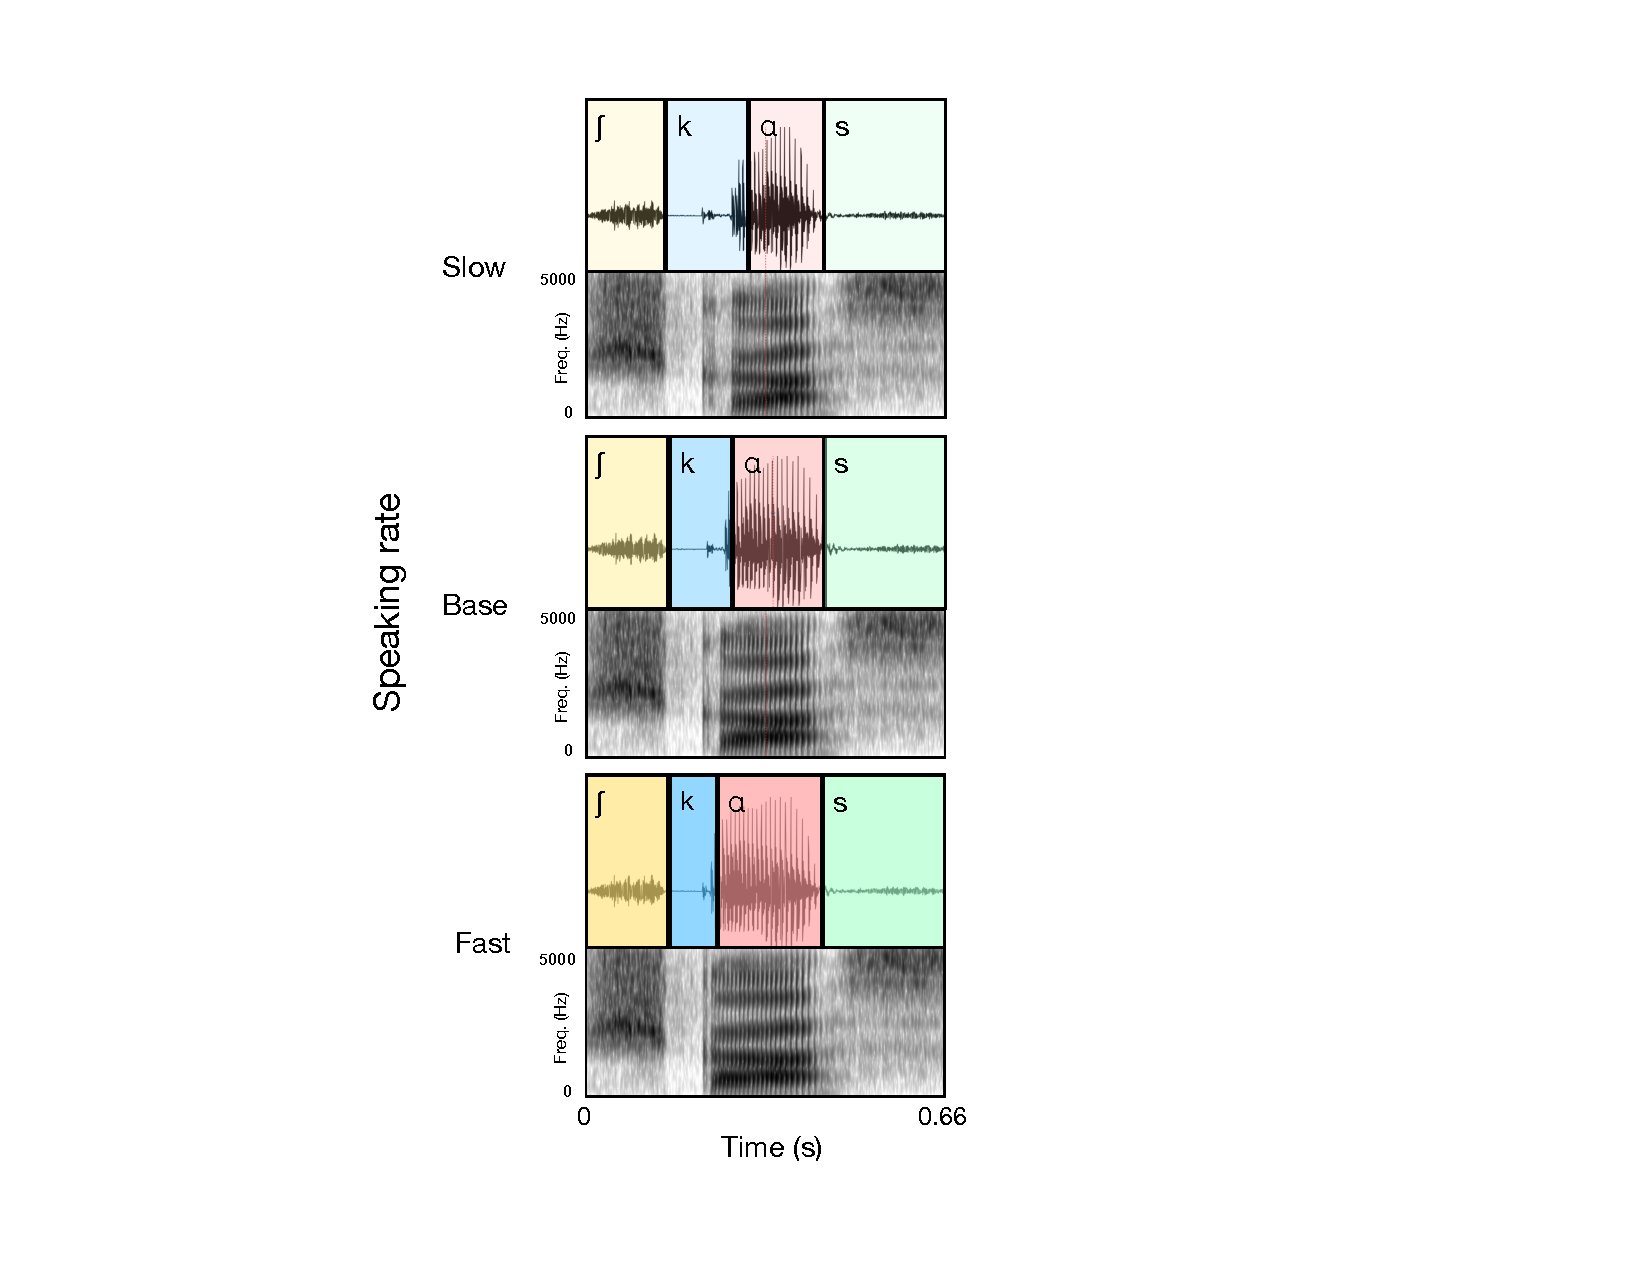
\includegraphics[scale=.75]{figures/stimuli_schema.pdf}
\caption{\label{fig:schema-exp1}} Speaking rate manipulations and stimuli duration for first step of series: Experiment 1. 
\end{figure}

The duration of /k/ was altered by removing or reduplicating pitch pulses and sections of burst and aspiration. Only short, nonadjacent sections of burst and aspiration were deleted or reduplicated so as to maintain the general amplitude profile and prevent the perception of frozen noise. No change was made to the closure duration; although closures do tend to vary slightly with speaking rate, this variability is typically quite small \citep{crystalSegmentalDurationsConnected1988,gayEffectSpeakingRate1978}, and thus unlikely to have a substantial perceptual effect. For the short /k/ stimulus, two pitch pulses were removed, as well as 17.2 ms of the burst and aspiration; for the long /k/ stimulus, four pitch pulses and 22 ms of the burst and aspiration were reduplicated. The vowel duration was similarly adjusted by removing or reduplicating nonadjacent pitch pulses, so as to make the absolute amount of change in the vowel as close as possible to the absolute amount of change in the stop consonant. The original /k/ stimulus served as the intermediate duration stimulus resulting in a 3-way /k/-duration series (short/fast, baseline/intermediate, and long/slow), although we make no claims as to it actually being half-way between the other two stimuli perceptually. The short /k/, base /k/, and long /k/ versions of the syllable were then appended to each member of the 10-item /\textesh/-/t\textesh/ series. 

\paragraph{Procedure}

Participants completed 1 practice/training block of 60 trials and 4 test blocks of 90 trials each. Responses from the training block were not analyzed. The four 90-trial test blocks were comprised of three repetitions of each of the 30 stimuli (3 /k/ durations X 10-step /\textesh-t\textesh/ continuum) for a total of 360 trials per participant, or 12 repetitions of each stimulus. 

Stimuli within each block were presented randomly to listeners using a Macintosh 7100/AV computer at a comfortable listening level over Audiotechnica ATH-M40 headphones. Listeners were prompted with each stimulus and asked to rate the quality of the initial phoneme on a six-point scale, ranging from ``a good \textit{sh}'' to ``a good \textit{ch}'', by pressing the appropriate button on a computer-controlled response box. The use of ratings allowed the detection of subtle differences within a category that may not have been obvious with simpler, categorical labeling \citep{sawuschSelectiveAdaptationEffects1976}. Presentation pace depended on the subject's response rate. Each trial began 1000 ms after the listener had responded to the previous trial, or after an interval of 3000 ms following stimulus onset, whichever came first. The experiment lasted approximately 45 minutes. 

\subsection{Results}

Data were analyzed in the RStudio computing environment (version: 1.4.1103; \citealt{rstudioteamRStudioIntegratedDevelopment2020}). Visualizations were created with \texttt{ggplot2} \citep{wickhamGgplot2ElegantGraphics2016}. Modeling was conducted and presented using the \texttt{lme4} \citep{batesFittingLinearMixedeffects2015}, \texttt{lmerTest} \citep{kuznetsovaLmerTestPackageTests2017}, and \texttt{broom.mixed} \citep{bolkerBroomMixedTidying2020} packages. Model parameter significance was determined via a combination of log-likelihood comparisons between models, AIC estimations, and p-values from model summaries.  

To test for an effect of phoneme duration on rate normalization, we modeled two different outcome variables: percentage of /\textesh/ responses and /\textesh/-ness ratings. For the percentage of /\textesh/ responses, an average /\textesh/ response was calculated for each participant, for each stimulus item (Figure \ref{fig:exp1-response-function}), while /\textesh/-ness ratings were simply computed for each individual stimulus item presented (item-level effect) (Figure \ref{fig:exp1-eshness-rating}). We elected to model two outcomes because traditional work on rate normalization has modeled percentage phoneme responses grouped over stimuli repetitions (e.g. \citealt{diehlAuditoryBasisStimulus1989}), while newer work has been able to model item-level effects (e.g. \citealt{maslowskiHowTrackingHabitual2019}) and we wished to make our work comparable to both of these domains.

\begin{figure}[H]
\centering
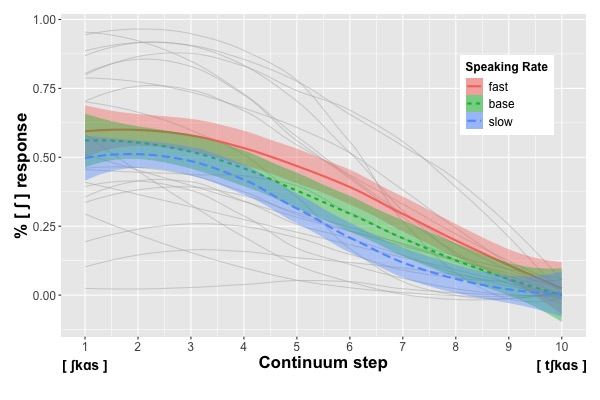
\includegraphics[scale=.5]{figures/exp1-percen.jpeg}
\caption{\label{fig:exp1-response-function} Spaghetti plot of percentage /\textesh/ response by series step and speaking rate: /k/ duration manipulation. Thick, darker lines represent group averages by speaking rate and lighter lines represent individual participant responses. Ribbons represent 95\% confidence intervals.}
\end{figure}

Figures \ref{fig:exp1-response-function} and \ref{fig:exp1-eshness-rating} suggest the presence of a rate normalization effect from phoneme duration manipulations. The confidence intervals surrounding the speaking rate conditions (Slow, Base, Fast) do not overlap in the middle, ambiguous section of the continuum. More specifically, we see the effect in the expected direction: slower speaking rates bias /t\textesh/ responses and higher /t\textesh/ ratings, while faster rates bias /\textesh/ responses and higher /\textesh/ ratings.

\begin{figure}[H]
\centering
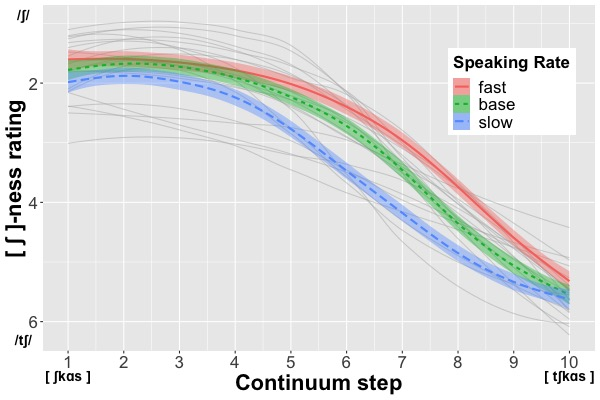
\includegraphics[scale=.5]{figures/exp1-eshness-rating.jpeg}
\caption{\label{fig:exp1-eshness-rating} Spaghetti plot of /\textesh/-ness ratings (1=good /\textesh/, 6=good /t\textesh/) by series step and speaking rate: /k/ duration manipulation. Thick, darker lines represent group averages by speaking rate and lighter lines represent individual participant responses. Ribbons represent 95\% confidence intervals.}
\end{figure}

To further examine a potential rate normalization effect, we fit models to our two outcome variables. Both models were fit to ambiguous items in the middle of the stimuli series, at the categorical perception boundary (steps 4-7 in this continuum, following \citet{bidelmanAcousticNoiseVision2019} who modeled steps 3-5 on a 7-point continuum). To predict the percentage of /\textesh/ responses, we fit a linear mixed effects model with the maximal random effect structure that permitted model convergence. This model included random slopes of Speaking Rate by Participant. Slope terms for interactions of Speaking Rate and Continuum Step did not converge, nor did models with random intercepts of Participant together with slopes of Speaking Rate by Participant. The effect of Speaking Rate (modeled categorically as ``Slow,'' ``Base,'' and ``Fast'') improved upon the random effects-only model as did Continuum Step (modeled as a continuous variable) (Table \ref{tab:exp1-sh-percen-model-summary}).\footnote{In the random effects, Continuum Step was modeled as three-way categorical variable; these models did not converge.} Unsurprisingly, the percentage of /\textesh/ responses decreased with increased steps along the continuum (\(\beta\)=-0.09, z=-12.15, p\textless.001). For Speaking Rate, there was a higher percentage of /\textesh/ responses in the Fast condition than the Base condition (\(\beta\)=0.09, z=3.72, p=0.001) and a lower percentage of /\textesh/ responses in the Slow condition than Base (\(\beta\)=-0.07, z=-2.54, p=0.019), suggesting a rate normalization effect.

\begin{table}
\caption{\label{tab:exp1-sh-percen-model-summary}Model predicting percentage /\textesh/ response: Experiment 1}
\centering
\begin{tabular}[t]{lrrrrl}
\hline\noalign{\smallskip}
Parameter & Estimate & S.E. & z-statistic & p-value & 95\% CI\\
\hline\noalign{\smallskip}
Intercept & 0.56 & 0.06 & 9.86 & <.001 & 0.45 - 0.67\\
Rate:Fast & 0.09 & 0.02 & 3.72 & 0.001 & 0.04 - 0.14\\
Rate:Slow & -0.07 & 0.03 & -2.54 & 0.019 & -0.12 - -0.02\\
Continuum Step & -0.09 & 0.01 & -12.15 & <.001 & -0.1 - -0.07\\
\hline\noalign{\smallskip}
\end{tabular}
\end{table}


To model item-level effects, we fit a second model to predict /\textesh/ ratings (1-6 scale where a lower rating indicates more /\textesh/-ness and a higher rating indicates more /t\textesh/-ness). The random effect structure again included the maximal number of terms that permitted model convergence, in this case random effects of Participant and Item. There were significant main effects of Continuum Step and Speaking Rate (Table \ref{tab:exp1-sh-rating-model-summary}). Ratings increased with continuum steps, indicating increased perception of /t\textesh/ (\(\beta\)=0.50, z=10.79, p<.001). Most importantly, the Slow speaking rate condition predicted higher ratings, or more /t\textesh/-ness, than the Base speaking rate condition (\(\beta\)=0.59, z=4.67, p=.005): a longer /k/ duration, suggesting a slower speaking rate, biased listeners to perceive and rate the stimuli as more /t\textesh/-like. However, there was only a reliable effect of Speaking Rate in the Slow condition; the difference between the Fast and Base speaking rates upon listeners' rankings approached but did not reach significance.

\begin{table}
\caption{\label{tab:exp1-sh-rating-model-summary}Model predicting /\textesh/-ness ratings: Experiment 1}
\centering
\begin{tabular}[t]{lrrrrl}
\hline\noalign{\smallskip}
Parameter & Estimate & S.E. & z-statistic & p-value & 95\% CI\\
\hline\noalign{\smallskip}
Intercept & 1.31 & 0.18 & 7.16 & <.001 & 0.95 - 1.66\\
Rate:Fast & -0.27 & 0.13 & -2.14 & 0.052 & -0.52 - -0.02\\
Rate:Slow & 0.59 & 0.13 & 4.67 & 0.005 & 0.34 - 0.84\\
Continuum Step & 0.50 & 0.05 & 10.79 & <.001 & 0.41 - 0.59\\
\hline\noalign{\smallskip}
\end{tabular}
\end{table}


Overall, these results demonstrate that manipulating /k/ duration, while holding the syllable duration constant, significantly affected the percentage of /\textesh/ responses and /\textesh/-ness ratings, especially in the Slow speaking rate condition, suggesting that listeners can normalize for speaking rate over individual phonemes.

\subsection{Interim discussion}

Experiment 1 demonstrated that two phonemes with obvious acoustic boundaries, /k/ and /\textscripta/, were treated as separate units during rate normalization. This result implies that the processing unit during rate normalization is something smaller than a syllable. However, /k/ and /\textscripta/ are fairly acoustically distinct and easy to distinguish from one another. Do listeners scale for speaking rate over phoneme-sized units that are difficult to distinguish? Experiment 2 examines a syllable containing phonemes that are much more difficult to segment acoustically: a glide and a vowel. To examine this, we chose a nonce word series that ranged from /\textesh w\textsci b/-/t\textesh w\textsci b/. Previous work on similar stimuli---a /sw\ae b/-/tw\ae b/ continuum---demonstrated that varying the /w/ duration while leaving the vowel constant, and varying the /\ae/ duration while leaving the glide constant, both lead to a change in category boundary location for the initial /s-t/ contrast \citep{newmanPerceptualNormalizationSpeaking1996}. Yet the effect could have been driven by the duration of a unit larger than the phoneme, because changing the /w/ duration while leaving the /\ae/ constant results in the combined syllabic unit also being longer. However here, as in Experiment 1, we varied the /w/ duration while also altering the /\textsci/ duration in the opposite direction, leading once again to a series with consistent syllable and word durations. If /w/ and /\textsci/ are treated as separate units during rate normalization, as /k/ and /\textscripta/ were, then manipulating the duration of /w/ should lead to a rate normalization effect in this series. 

\section{Experiment 2}\label{exp2}

\subsection{Methods}

\paragraph{Participants}

Twenty-two members of the University of Iowa community participated in this experiment for course credit. All were native English speakers with no reported history of a speech or hearing impairment. Three participants did not respond on at least 80\% of the trials, so their data were removed from analysis leaving 19 participants. 

\paragraph{Stimuli}

Stimulus creation was nearly identical to that in Experiment 1. The same speaker produced the syllable /\textesh w\textsci b/ in the same manner previously described. The initial fricative was separated from the remainder of the syllable, with the boundary being the zero-crossing preceding the first pitch pulse of the /w/. A series of ten items ranging from /\textesh/ to /t\textesh/ was created in a similar manner as Experiment 1, by removing successive sections of approximately 10 ms from the onset of the /\textesh/. 

The syllable /w\textsci/ was edited in the same manner as the /k\textscripta/ syllable in Experiment 1. Based on spectral analysis, the first 7 vocal pulses were considered part of /w/ rather than the /\textsci/, because these pulses appeared to constitute the /w/ formant transitions (especially those of the first formant). We lengthened and shortened the /w/ and /\textsci/ durations by reduplicating or deleting nonadjacent pitch pulses in the same manner as before. For the shorter /w/, three pitch pulses were removed, whereas four pulses were reduplicated to create the long /w/ (and pitch pules from the vowel were likewise removed or reduplicated in the same manner to keep the syllable duration constant). The original items served as the intermediate duration. The /w/ duration was shorter than that of the /\textsci/, so the same amount of absolute change resulted in a larger change proportionately for the /w/ than for the vowel. The short /w/, baseline/intermediate /w/, and long /w/ versions of the syllable were then appended to each member of the 10-item /\textesh/-/t\textesh/ series. This resulted in three /w/-duration series with a constant syllable and word duration, but varying /w/ (and vowel) durations.

\begin{figure}
\centering
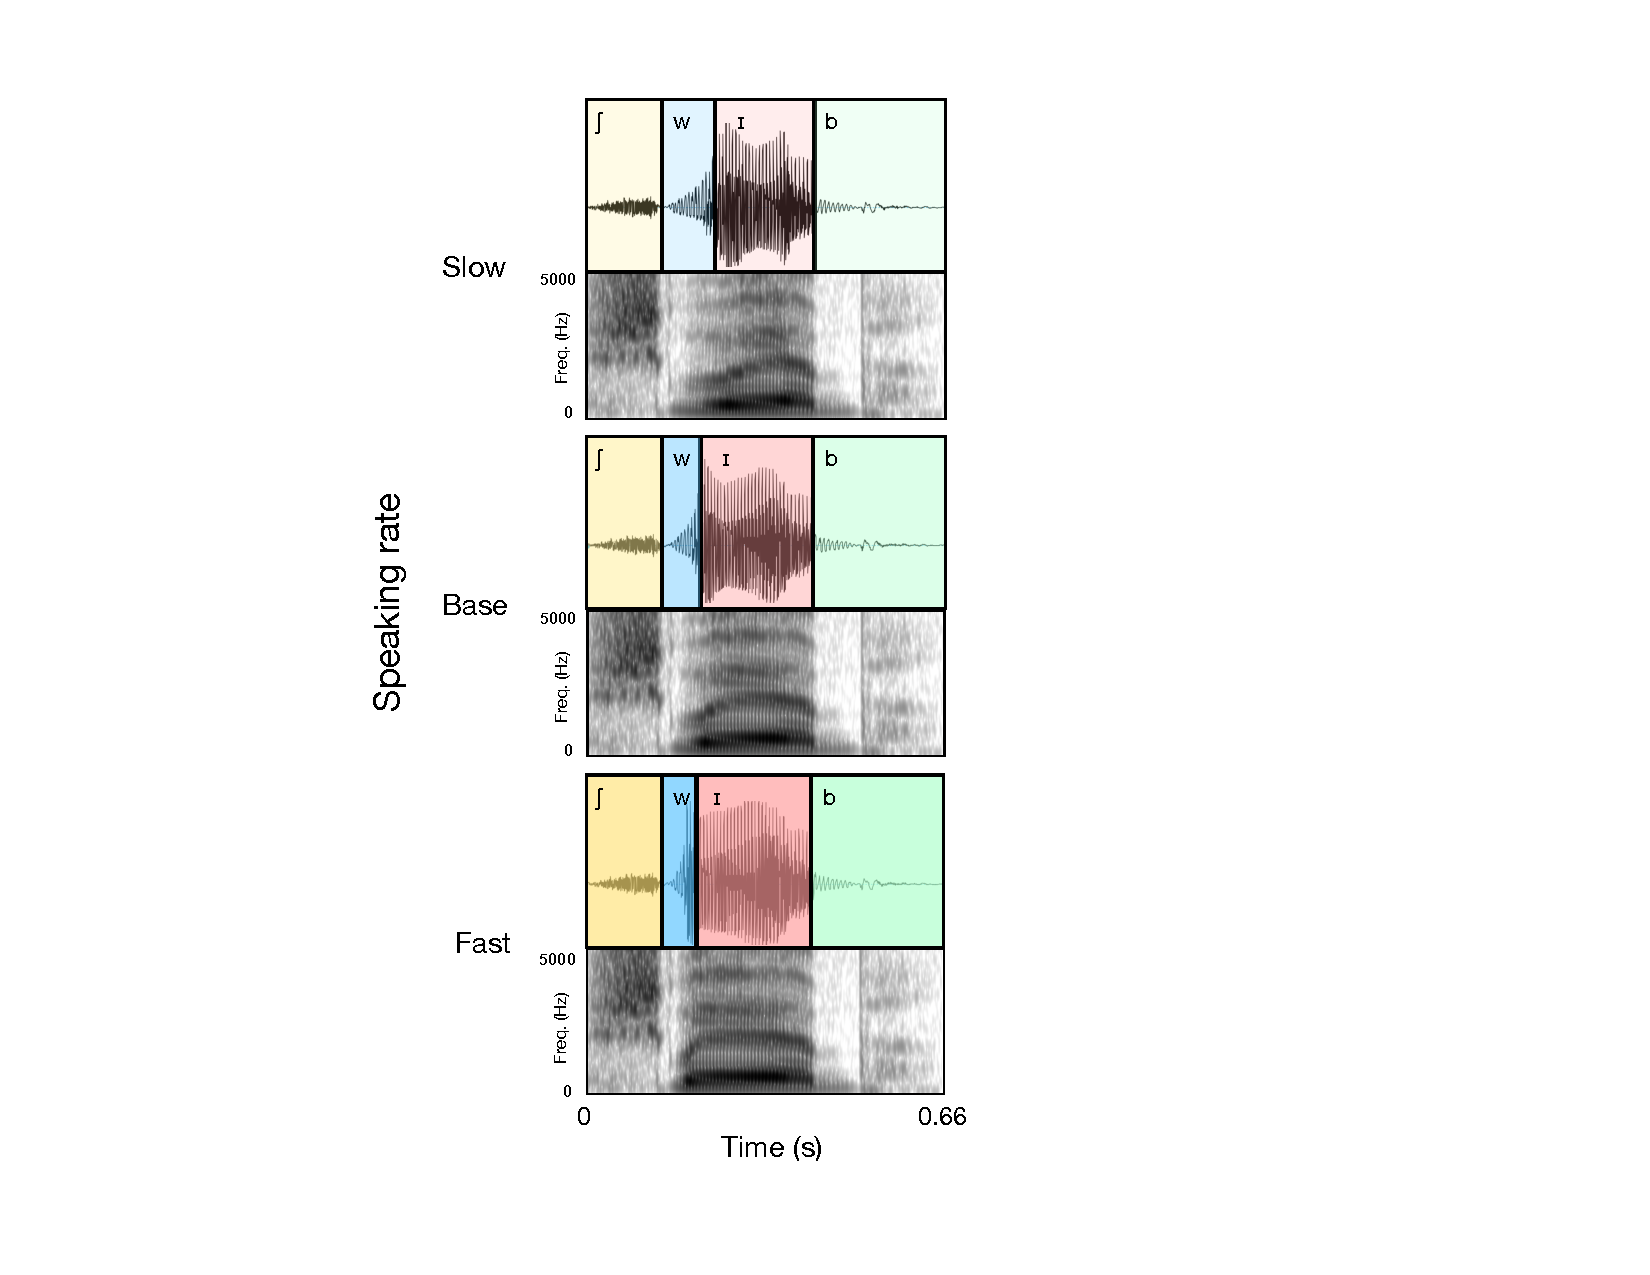
\includegraphics[scale=.75]{figures/stimuli_schema_exp2.pdf}
\caption{\label{fig:schema}} Speaking rate manipulations and stimuli duration for first step of series: Experiment 2. 
\end{figure}

% The following is text from the original experiment on s-t contrast; we need raw recordings of speech stimuli to fix this paragraph if we want to be able to say these things
%As shown in Table 2, the amount of change in absolute values for the consonant /w/ is slightly smaller than that for the /k/ in the previous experiment (27 msec vs. 32 msec for shortening, and 36 msec vs. 50 msec for lengthening).  However, the base /w/ duration was shorter than that of the /k/ duration in Experiment 1, so this change is actually larger proportionately.  Given that this amount of proportional change was sufficient to instigate rate normalization in the prior experiment, it should be sufficient here as well.  Thus, if the /w/ and vowel are treated as separate segments by the rate normalization process, we would expect to find the same shift in perception of the initial sound as was found in the prior study.

\paragraph{Procedure}

The procedure was identical to that of Experiment 1.

\subsection{Results}

As in Experiment 1, to evaluate a potential rate normalization effect we modeled two different outcome variables: percentage of /\textesh/ responses and /\textesh/-ness ratings. Again, an average /\textesh/ response was calculated for each participant (Figure \ref{fig:exp2-response-function}) and /\textesh/-ness ratings were computed for each individual stimulus (Figure \ref{fig:exp2-eshness-rating}). The visualizations suggest an effect of speaking rate (/w/ duration) upon /\textesh/ responses and /\textesh/ ratings in the same direction as Experiment 1: slower speaking rates bias more /t\textesh/ responses.

\begin{figure}[htpb]
\centering
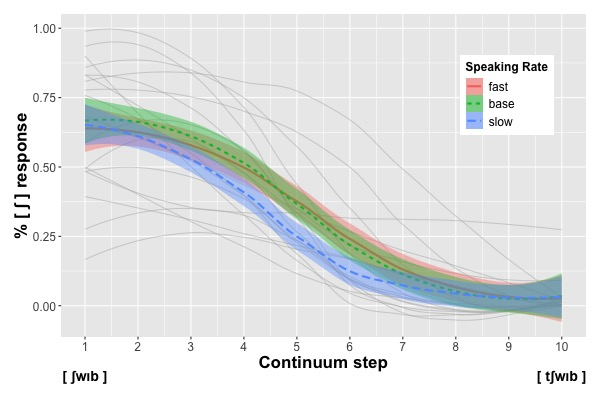
\includegraphics[scale=.5]{figures/exp2-percen.jpeg}
\caption{\label{fig:exp2-response-function}Spaghetti plot of percentage /\textesh/ response by series step and speaking rate: /w/ duration manipulation. Thick, darker lines represent group averages by speaking rate and lighter lines represent individual participant responses. Ribbons represent 95\% confidence intervals.}
\end{figure}

\begin{figure}
\centering
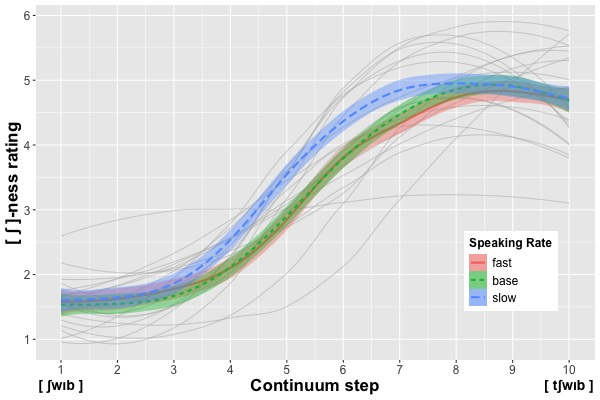
\includegraphics[scale=.5]{figures/exp2-eshness-rating.jpeg}
\caption{\label{fig:exp2-eshness-rating}Spaghetti plot of /\textesh/-ness ratings (1=good /\textesh/, 6=good /t\textesh/) by series step and speaking rate: /w/ duration manipulation. Thick, darker lines represent group averages by speaking rate and lighter lines represent individual participant responses. Ribbons represent 95\% confidence intervals.}
\end{figure}

As before, we fit a series of models to the ambiguous items in the middle of the stimuli series, at the categorical perception boundary (steps 4 through 7). To predict the percentage of /\textesh/ responses, we fit a linear mixed effects model that included random slopes of Speaking Rate by Participant. Like Experiment 1, there were significant main effects of Speaking Rate and Continuum Step: the percentage of /\textesh/ responses increased as the continuum step increased (more /t\textesh/-like stimuli) (\(\beta\)=-0.13, z=-14.44, p\textless.001). There was a significantly smaller percentage of /\textesh/ responses in the Slow speaking rate condition than Base condition (\(\beta\)=-0.09, z=-2.66, p=0.02), demonstrating a rate normalization effect for these stimuli, but no difference in the percentage of /\textesh/ responses between the Fast speaking rate condition and the Base condition (Table \ref{tab:exp2-sh-percen-model-summary}).

\begin{table}
\caption{\label{tab:exp2-sh-percen-model-summary}Model predicting percentage /\textesh/ response: Experiment 1}
\centering
\begin{tabular}[t]{lrrrrl}
\hline\noalign{\smallskip}
Parameter & Estimate & S.E. & z-statistic & p-value & 95\% CI\\
\noalign{\smallskip}\hline\noalign{\smallskip}
Intercept & 1.00 & 0.07 & 15.33 & <.001 & 0.88 - 1.13\\
Rate:Fast & 0.02 & 0.02 & 0.69 & 0.49 & -0.03 - 0.06\\
Rate:Slow & -0.09 & 0.03 & -2.66 & 0.02 & -0.16 - -0.02\\
Continuum Step & -0.13 & 0.01 & -14.44 & <.001 & -0.15 - -0.11\\
\noalign{\smallskip}\hline
\end{tabular}
\end{table}


Finally, we fit a model to predict /\textesh/-ness ratings for these stimuli, where a lower rating indicated that listeners considered the stimuli more /\textesh/-like. The random effect structure again included random intercepts by Participant and Item and there were significant main effects of Continuum Step and Speaking Rate (Table \ref{tab:exp2-sh-ness-model-summary}). Unsurprisingly, stimuli further along the /\textesh-t\textesh/ continuum were perceived as more /t\textesh/-like (\(\beta\)=0.82, z=17.66, p\textless.001). Longer /w/ durations, indicating a slower speaking rate, also biased listeners to perceive the stimuli as more /t\textesh/-like (\(\beta\)=0.54, z=4.20, p=.003). As with Experiment 1, we did not find an effect of speaking rate in the Fast speaking rate condition. Overall, the results from Experiment 2 show an effect of speaking rate (/w/ duration) upon the perceived phonetic boundary between /\textesh/ and /t\textesh/, indicating that normalization can occur over these phonemes without clear acoustic boundaries.

\begin{table}
\caption{\label{tab:exp2-sh-ness-model-summary}Model predicting /\textesh/-ness ratings: Experiment 2}
\centering
\begin{tabular}[t]{lrrrrl}
\hline\noalign{\smallskip}
Parameter & Estimate & S.E. & z-statistic & p-value & 95\% CI\\
\noalign{\smallskip}\hline\noalign{\smallskip}
Intercept & -1.19 & 0.30 & -3.99 & 0.002 & -1.78 - -0.61\\
Rate:Fast & -0.06 & 0.13 & -0.49 & 0.64 & -0.31 - 0.19\\
Rate:Slow & 0.54 & 0.13 & 4.20 & 0.003 & 0.29 - 0.79\\
Continuum Step & 0.82 & 0.05 & 17.66 & <.001 & 0.73 - 0.91\\
\noalign{\smallskip}\hline
\end{tabular}
\end{table}


\section{General discussion}

Listeners must compensate for variation across different speakers, in different contexts, to comprehend speech and language. Normalization for speaking rate is one important example of this process: it allows listeners to maintain temporal contrasts, such as voice onset time, across different speech speeds and between different speakers. In a pair of experiments, we evaluated whether listeners could use information from individual phonemes---which coarticulation and hypoarticulation often render undefined in the acoustic signal---instead of syllables to normalize for speaking rate. Listeners did normalize over phonemes, including acoustically-overlapping phonemes, to factor out speaking rate, demonstrating that the phoneme is a potential processing unit for rate normalization processes.

Work on proximal information in the speech signal for rate normalization has long suggested that normalization occurs over individual phones \citep{diehlAuditoryBasisStimulus1989,newmanPerceptualNormalizationSpeaking1996}. Empirical support was lacking, however, because previous work altered the duration of the carrier syllable and word in addition to the phone. Here we compensated for changes in consonant duration by also changing the nucleus duration. This step allowed us to maintain a consistent syllable duration, avoid the previous experimental confound, and isolate effects of phoneme duration on rate normalization. Since we replicated previous work in finding an effect of phoneme duration on this phonetic boundary shift, we can now more definitively say that listeners can use phonemes to compute speaking rate. Furthermore, by also evaluating the effects of acoustic distinctiveness on rate normalization, we were additionally able to show that this phoneme processing for rate normalization even occurs in less-than-ideal acoustic environments. 

Rate normalization can be activated after just milliseconds of exposure \citep{reinischSpeakerspecificProcessingLocal2016}, and is documented in human and non-human species alike \citep{welchEffectsSyllablefinalSegment2009}, suggesting that this type of normalization is a low-level auditory process that could be partially domain-general. Finding that listeners can compute speaking rate over individual phonemes speaks directly to this idea. Phonemes do not relay a clear acoustic signal. They are indistinct, coarticulated, and reduced---traits that are exacerbated when the features (voicing, stridency) of adjacent phones overlap within syllables. If rate normalization were exclusively or primarily domain-general, it is unclear how listeners could normalize over individual phonemes. It is possible that listeners may \textit{prefer} or \textit{tend} to normalize over syllables, or relatively more acoustically-reliable components of speech such as word boundaries, but will compute over phonemes in the absence of higher-level information. Our experiments were not designed to contrast listeners' preferred processing unit for rate normalization. It is also possible, as \citet{boskerAccountingRatedependentCategory2017} suggests, that perceptual normalization for speaking rate could be domain general for some lower-level constructs, such as phonetic boundary shifts, but increasingly language-specific at higher levels such as determining the presence of function words \citep{dilleyAlteringContextSpeech2010}. Nevertheless, the fact that listeners could normalize over phonemes in these experiments is strong evidence that rate normalization processes are driven by experience with a language, instead of the raw acoustic signal alone. 

The results of these experiments open up several avenues for future research. First, these experiments only tested American English listeners listening to mostly singleton consonants and monophthongal vowels embedded in nonce words. But other works have found clear effects of language structure and experience on rate normalization \citep{baese-berkNonnativeSpeakersUse2016,steffmanIntonationalStructureMediates2019}. Do listeners also normalize over units, like morae, geminates, or diphthongs that are heavier/larger than phonemes but smaller than syllables? Phonotactic structure is another unexplored aspect of language structure that may be relevant for understanding how listeners calculate speaking rate. Some languages, such as Japanese, tend to have more acoustically ``confusable'' internal syllable structures, only permitting nasal consonants, and not stops, in coda position for example. If the acoustic signature within syllables tends to be more indistinct, listeners could learn to rely less on individual phonemes for normalization. Studying how perceptual normalization for speaking rate develops in children would be another way to evaluate this idea. 

It will also be important for future work to evaluate processing units for normalization in faster and more naturalistic stimuli as perceptual normalization for speaking rate is likely idiosyncratic and dependent upon the context and speaker \citep{goldingerPuzzlesolvingScienceQuixotic2003}. And more naturalistic stimuli, that contain multiple, co-varying phonetic cues (i.e formant transition duration and frequency), have previously been shown to mitigate rate normalization effects \citep{shinnLimitationsContextConditioned1985}. Here we originally hypothesized that listeners would normalize over syllables or other supra-phonemic chunks because phonemes are highly confusable and indistinct during comprehension especially in fast, running speech. And while our experiments instead showed reliable effects of phoneme duration on the phonetic boundary shift, the experimental stimuli clearly differed from what listeners would hear and process in real-world contexts. For example, even the manipulated consonant in the ``fast'' speaking rate condition in Experiment 1 was relatively slow (91 ms) compared to the word-medial stop consonants that listeners might hear in everyday conversation. For extremely fast speech, listeners might rely less on individual phones and more on syllables or words. Faster, naturalistic speech also drives acoustic reduction and heightened coarticulation \citep{fourakisTempoStressVowel1991,gayMechanismsControlSpeech1981}. However, these acoustic cues did not necessarily accompany the stimuli employed in these experiments as we wanted to isolate the effects of speaking rate. But extreme reduction in other, more naturalistic listening conditions could lead listeners to normalize over different units. 

\subsection{On cue integration versus normalization}

Some recent work on proximal cues for phoneme classification has suggested that listeners may not normalize for speaking rate but rather \textit{integrate} acoustic cues that overlap with speaking rate to classify phonemes \citep{toscanoCueIntegrationCategories2010,toscanoCueintegrationContextEffects2012}. For example, for voice onset time contrasts, vowel duration indicates both speaking rate and voicing: the burstiness of voiceless stops can cause the onset of the following vowel to de-voice slightly, leading it to be perceived as shorter in duration. 

While it was not the goal of this study to contrast cue integration and rate normalization accounts to explain proximal effects upon phonetic boundary shifts---and the results of \citet{toscanoCueintegrationContextEffects2012} do convincingly demonstrate that vowel length integration, not normalization for speaking rate, explains proximal effects upon stop voicing classifications---we believe the current results show rate effects and not the more straightforward acoustic cue integration. This is because our target contrast for both studies, /\textesh-t\textesh/, was cued by the duration of the following \textit{consonant}, not vowel (/k/ in /\textesh k\textscripta s/-/t\textesh k\textscripta s/ for Exp. 1 and /w/ in /\textesh w\textsci b/-/t\textesh w\textsci b/ for Exp. 2). But more importantly, there is no evidence that stop or glide duration reliably indicates fricative-affricate classification. And unlike the effect of stop aspiration upon perceived vowel length (aspiration causes vowel de-voicing), there is no phonetic reason to assume that fricatives and affricates would have different effects on /k/ or /w/ duration or voicing. Consequently, we believe that the effects of consonant duration upon the phonetic boundary shift between /\textesh/ and /t\textesh/ in these studies indicates rate normalization, not cue integration. 

\section{Conclusion}

Unlike previous work studying proximal effects on rate normalization, this study manipulated speaking rate via phoneme duration while holding the duration of carrier syllables and words constant. We still demonstrated rate effects upon the phonetic boundary shift between /\textesh/ and /t\textesh/, both for syllables containing acoustically-distinct /k\textscripta/ and -overlapping phonemes /w\textsci/. These results present evidence that listeners process speaking rate over individual phonemes, even in the absence of clear acoustic boundaries between phones, suggesting roles of linguistic structure and language experience for perceptual normalization of speaking rate.  



\begin{acknowledgements}
The authors wish to thank Jessica Burnham, Jim Sawusch, and Jan Edwards for their assistance with this work. 
\end{acknowledgements}

\section*{Data availability}
Analysis scripts to replicate modeling results are included in the affiliated GitHub repository (\url{https://github.com/megseekosh/rate-normalization}. Experiments were not pre-registered.

\section*{Conflict of interest}
The authors declare that they have no conflicts of interest.


% BibTeX users please use one of
\bibliographystyle{apalike}
\bibliography{My_Library}   % name your BibTeX data base

\end{document}

